\documentclass[a4paper]{article}

\usepackage[utf8]{inputenc}
\usepackage{erk}
\usepackage{times}
\usepackage{graphicx}
\usepackage[top=22.5mm, bottom=22.5mm, left=22.5mm, right=22.5mm]{geometry}

\usepackage[slovene,english]{babel}
\usepackage{hyperref}
\usepackage{url}

\let\oldfootnotesize\footnotesize
\renewcommand*{\footnotesize}{\oldfootnotesize\scriptsize}

\begin{document}
\title{Poročilo za prvi seminar pri predmetu Računalniška grafika in tehnologija iger}

\author{Strahinja Đorđević$^{1}$, Natalija Ivanović$^{2}$, Nikola Kokotović$^{3}$ }

\affiliation{Univerza v Ljubljani, Fakulteta za računalništvo in informatiko}

\email{	$^{1}$E-pošta: st41384@student.uni-lj.si \\ 
				$^{2}$E-pošta: ni8490@student.uni-lj.si  \\
                $^{3}$E-pošta: nk37190@student.uni-lj.si}

\maketitle

\selectlanguage{slovene}

\begin{abstract}{Abstract}
Ime igre je Ajda Simulator. Igra predstavlja simulacijo ljubljanske restavracije Ajda.
Cilj igre je zadovoljiti čim več strank v čim krajšem času, pri čemer mora igralec paziti na pravilno pripravo jedi in pravočasno dostavo.  
Igra je primerna za vse, ki uživajo v simulacijskih igrah in želijo preizkusiti svoje sposobnosti v vlogi kuharja.
\end{abstract}

\section{Pregled igre}
Igralec prevzame vlogo kuharja, ki mora sprejemati naročila, jih dostaviti strankam in pobirati denar.
Igra je povprečno zahtevna, za ljudje od 7 do 107 let.
Igralec na začetku od natakarja prevzame naročilo, nato gre v kuhinjo, kjer pripravi naročeno jed. Ko je jed pripravljena, jo dostavi stranki in pobere denar.
Kuhar se mora zelo dobro organizirati kako bi čim več strank zadovoljil v čim krajšem času.
Vsaka narejena jed prinese določeno število točk, ki se seštevajo na koncu igre.

\subsection{Opis sveta}
Svet igre je zasnovan kot kuhinja v restavraciji Ajda, kjer se odvija večina dogajanja. Model kuhinje je realističen, vendar ni povsem enak kuhinji omenjene restavracije. 
V svetu se nahajajo štiri sobe: omenjena kuhinja, shramba, soba za smeti in restavracija. Svet je zaprt, tako da igralec ne more zapustiti stavbe.
Osebki se premikajo v treh dimenzijah.

\subsubsection{Pregled}
Igralec se nahaja v kuhinji in interaktira z natakarjem, in predmeti v kuhinji. Od natakrja prevzame naročilo, nato gre v kuhinjo, kjer pripravi naročeno jed. 
Za pripravo jedi uporablja razne naprave, ki se nahajajo v kuhinji. Predmeti v kuhinji so štedilnik, friteza, zamrzovalnik, hladilnik in smeti. 
Kuhar tudi mora vzeti potrebne sestavine iz hladilnika in shrambe za pripravo jedi. Na voljo so mu: meso, zelenjava, pomfrit, kruh in Coca-Cola.

\subsubsection{Ozadje}
Ozadje igre predstavlja prostor za stranke restavracije Ajda, kjer se nahajajo mize in stoli.

\subsubsection{Ključne lokacije}
Ključne lokacije so natakarjev pult (kjer kuhar prevzame naročilo), shramba (kjer kuhar lahko najde kruh), zamrzovalnik (kjer kuhar lahko najde meso), hladilnik (kjer kuhar lahko najde Coca-Colo in zelenjavo),
štedilnik (kjer kuhar lahko speče meso), friteza (kjer kuhar lahko speče pomfrit), delovna miza (kjer kuhar sestavi burger), in smeti (kamor kuhar odvrže odpadke). 

\subsubsection{Velikost}
Svet vsebuje 4 sobe - prostor za stranke, zamrzovalnik/shramba, kuhinja in smetišče. 

\subsubsection{Objekti}
V igri smo vključili različne ključne elemente, kot so kuhinjski aparati, hladilniki, mize, stoli, hrana, pijače in drugi predmeti. 
Večina teh elementov je bila prilagojena našim potrebam, vsak objekt pa je bil posebej uvožen in prilagojen. 
Dodatne teksture\footnote{\url{https://www.freepik.com}} in objekte\footnote{\url{https://www.cgtrader.com}}\footnote{\url{https://www.turbosquid.com}}\footnote{\url{https://sketchfab.com}} smo skrbno izbrali s spletnih mest.

\subsubsection{Čas}
Čas igre je pohitren, ena pljeskavica se peče 15 sekund.

\subsection{Igralni pogon in uporabljene tehnologije}
Od tehologij smo vporabili Blender za modeliranje 3D prostora, Figmo skupaj z HTMLom in CSSom za izdelavo vporabniškega vmesnika in Reapper za obdelavo zvoka.
Poleg omenjenih, smo uporabili WebGPU za izris scene, programski jezik JavaScript za logiko igre.

\subsection{Pogled}
Pogled predstavlja prvoosebni pogled, kjer igralec vidi kuhinjo iz oči kuharja. Igralec ima interakcijo z različnimi objekti, preko vmesnika Objection Detection, ki je zadolžen za logiko, ki nam pove v kateri objekt je pogled igralca usmerjen.
Potem se odvisno od objekta, sproži interakcija z vmesnikom Inventory. Igralec v Inventory dobi zaželjen predmet(hrana ali pijača), ali pa lahko vrže stran predmet, ki ga ne potrebuje.
Collision je pa implementiran v vmesniku Physics, ki nam pove, če je igralec trčil v objekt ali ne.

Predmeti določeni za interakcijo: 
- žar, ki omogoča pečenje mesa v določenem času
- natakar, (ki je v tej verziji igre predstavljen kot tabla za obvestila7naročila) ki omogoča igralcu da prevzame naročilo, ali ga izroči
- delovna miza, ki omogoča igralcu da iz določenih sestavin naredi naročilo

Poleg interakcije, implementirane so tudi animacije:
- pobiranje kruha
- pobiranje mesa z žara 
- dajanje pljeskavice na žar
- animacija dima ko je meso na žaru

Za izris scene, svetlobe, materialov in tekstur je uporabljen Shader, ki podatke dobi iz Unit Renderer-ja. Kar se tiče vporabniškega vmesnika, implementirane so funkcije za prikazovanje inventara pridobljenih točk,
timer-ja za pečenja mesa in recepta za trenutno naročilo. V vmesniku so tudi implementirane funkcije za predvajanje zvoka, ki se sproži ob določenih dogodkih v igri.

\section{Osebek}
Igralec prevzame vlogo samo kuharja, lahko ga premika po kuhinji, pobira predmete in jih uporablja. Lahko še od natakarja prevzame naročilo.

\section{Uporabniški vmesnik}
Uporabniški vmesnik predstavljajo invetar, ki prikazuje katere sestavine ima kuhar na voljo, trenutna naročila, ki jih mora kuhar pripraviti, število točk, ki jih je kuhar že zbral in čas pečenja mesa.

\section{Glasba in zvok}
Zvoki v igri so prevzeti s spleta\footnote{\url{https://freesound.org}}. Zvok obstaja za interakcijo z objekti, štedilnik, ko se meso peče, hod kuharja in ambientalni zvoki restavracije.
Pesma v ozadju se imenuje Canyon's joyride, naredil jo je pa slovenski glasbenik 08080\footnote{\url{https://08080.bandcamp.com/album/astro-disco}}.

\section{Gameplay}
Igra se začne z naročilom, ki ga kuhar prevzame od natakarja. Nato gre v kuhinjo, kjer pripravi naročeno jed. 
Ko je jed pripravljena, jo dostavi nazaj natakarju. Nato lahko prevzame novo naročilo. 
\begin{figure}[!htb]
    \begin{center}
        \includegraphics[width=\columnwidth]{kitchen.png}
        \caption{Kuhinja}

    \end{center}
\end{figure}
\begin{figure}[!htb]
    \begin{center}
        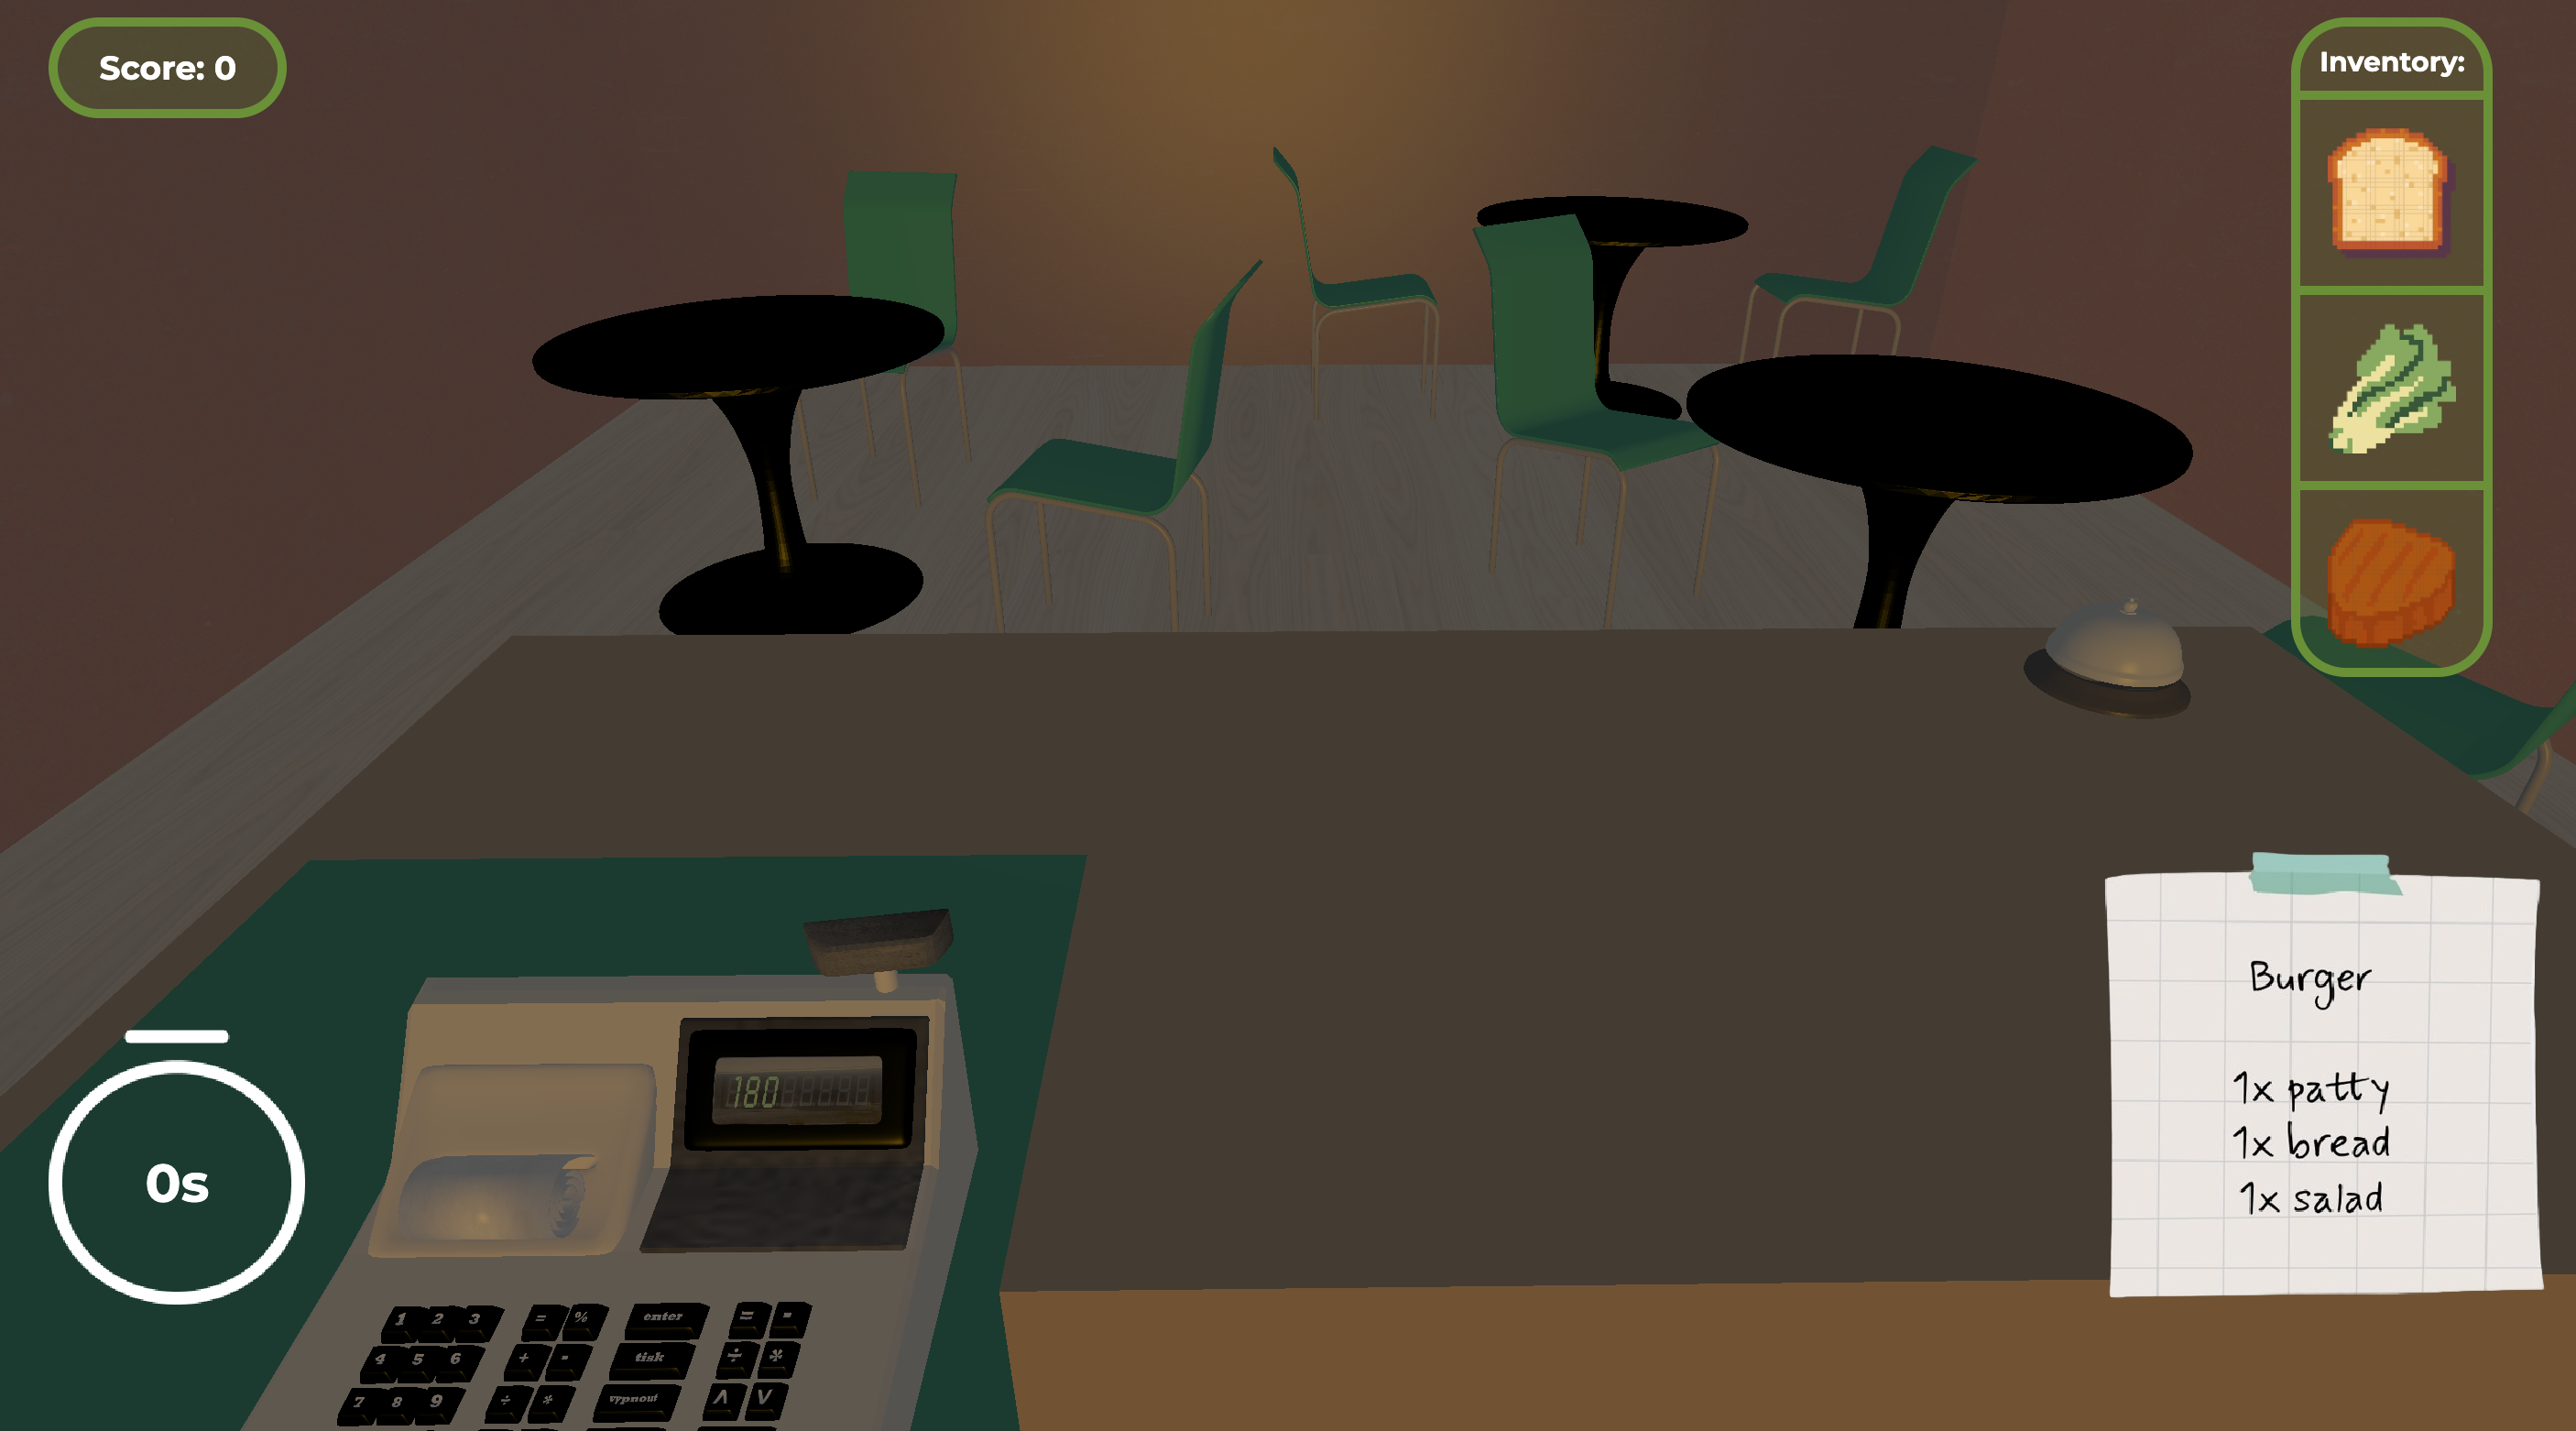
\includegraphics[width=\columnwidth]{restaurant.png}
        \caption{Restavracija}
    \end{center}
\end{figure}
\begin{figure}[!htb]
    \begin{center}
        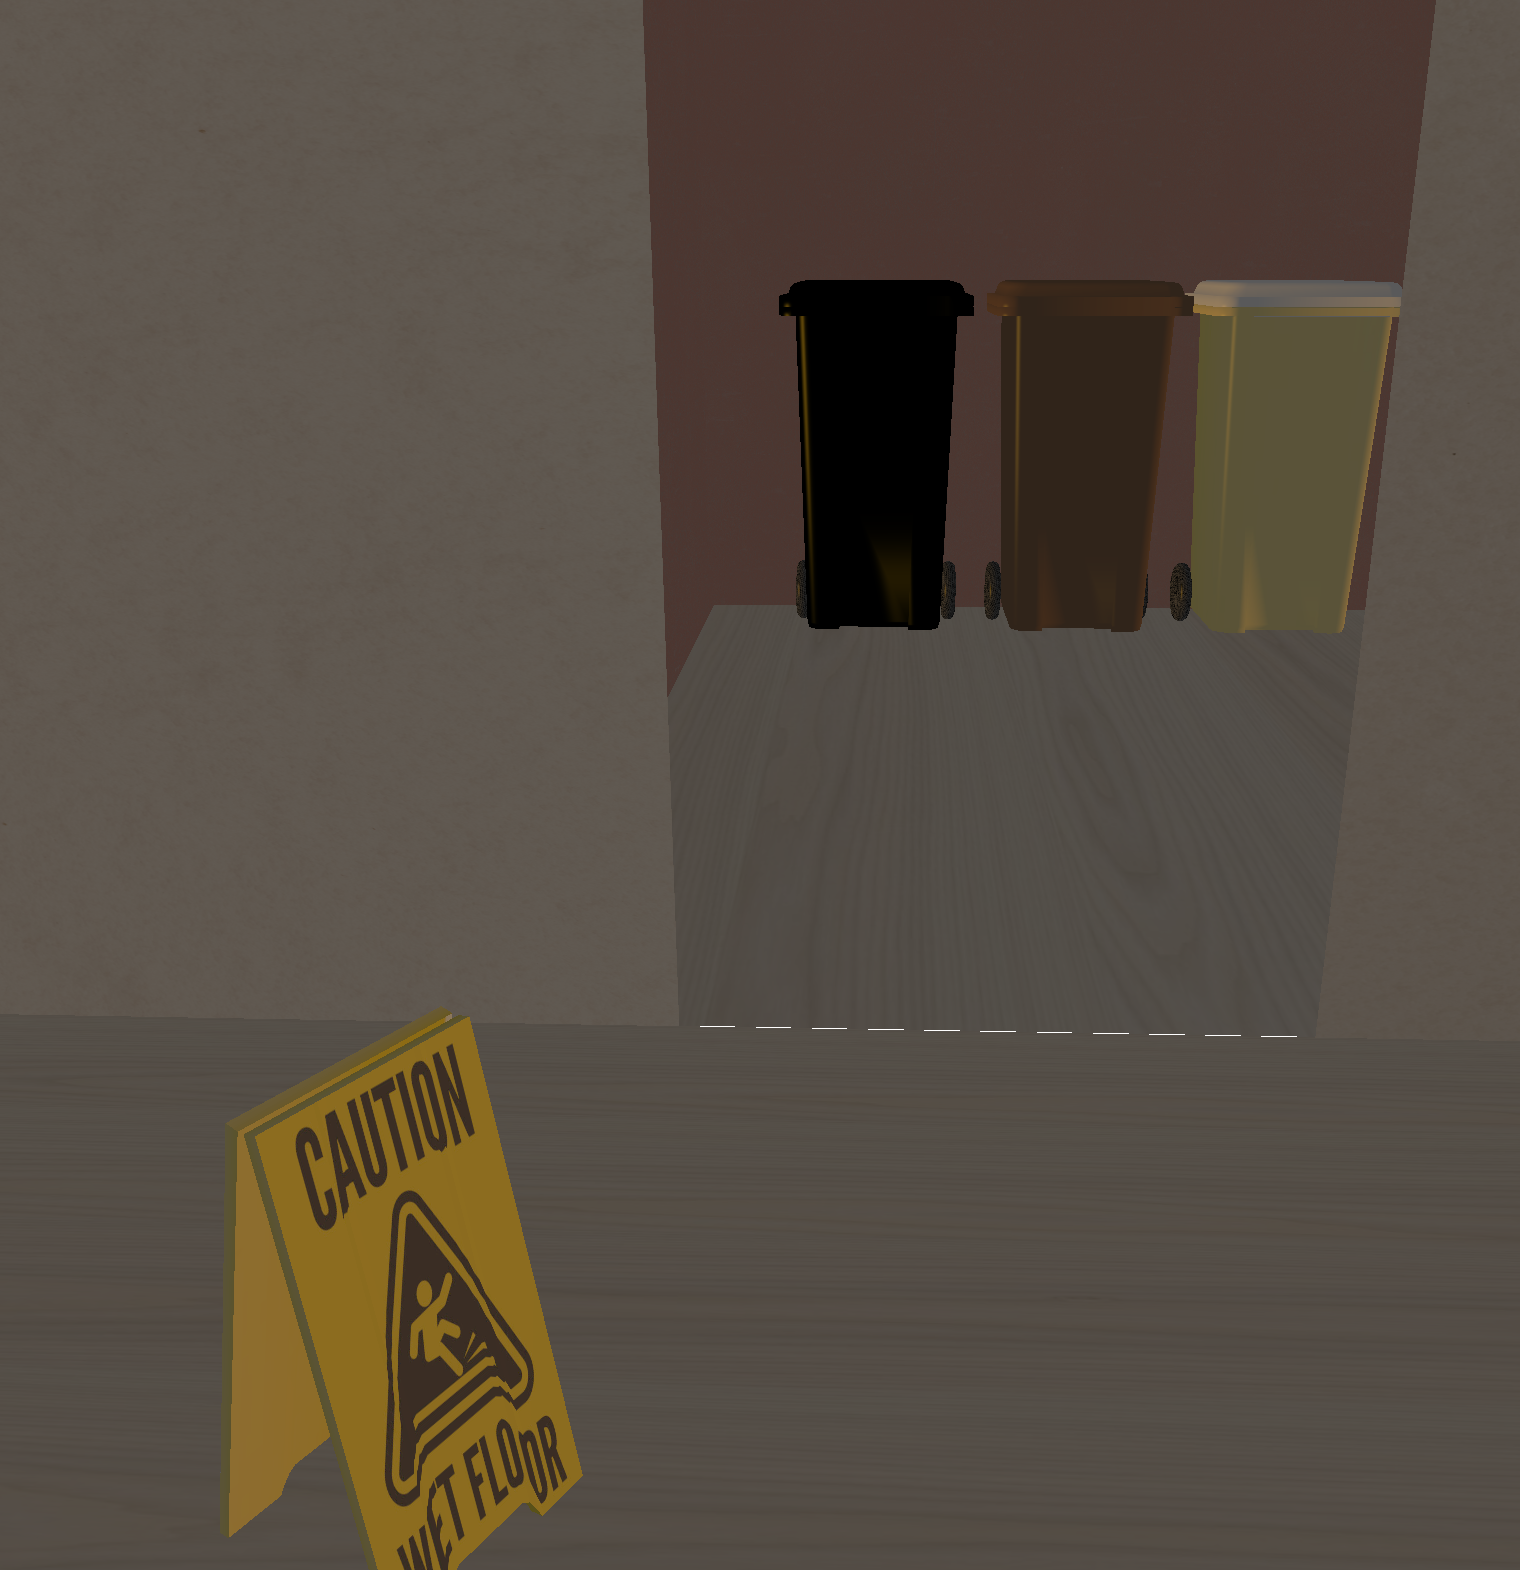
\includegraphics[width=\columnwidth]{wetFloor.png}
        \caption{Smetišče}
    \end{center}
\end{figure}

\section{Zaključki in možne nadgradnje}
Pri izdelavi igre smo se naučili tudi 3D modeliranja, kar nam je omogočilo boljše razumevanje oblikovanja in prilagajanja objektov v prostoru.
Razlike, do katerih je prišlo med začetnim načrtom in končno izvedbo, so se nanašale predvsem na vsebino jedilnega lista, ki smo ga sprva želeli narediti bolj obsežnega, ter na dodajanje še nekaterih objektov v končni model.
Končna izvedba igre je precej blizu prvotni zamisli, čeprav so tehnologije imele svoje omejitve. 
Ena od možnih nadgradenj bi bila dodajanje več igralcev v igro, ki bi lahko sodelovali pri pripravi jedi, ali igralca v ulogi natakarja, ki bi prevzemal naročila.
Radi bi tudi dodali večjo in bolj zanimivo kuhinjo, ki bi vsebovala prostorije kot so vinska klet, slaščičarna...

\small
\bibliographystyle{plain}
\bibliography{references}

\end{document}
